\section{Problem statement}
\label{sec:problem}

We first introduce three cold-start settings for playlist recommendation, 
then summarise recent work most related to recommend music to form playlists,
as well as music recommendation in cold-start scenarios.



\subsection{Three cold-start settings}

We investigate problems of recommending music to form playlists in three cold-start settings:
\begin{enumerate}[(i)]
\item \emph{cold songs}, where we recommend newly released songs to extend existing playlists;
\item \emph{cold playlists}, where we recommend a set of songs to form a new playlist for an existing user;
\item \emph{cold users}, where we recommend a set of songs to form a new playlist for a new user.
\end{enumerate}

%We address the three cold-start settings using one approach, namely, we first score each song 
%according to the given information (\eg an existing playlist, an existing user or a new user),
%%then we can form a playlist by either taking the top-K scored songs or sampling songs proportional to their scores.
%then take the top scored songs as our recommendation.
%Specifically, for the task of recommending newly released songs to extend an existing playlist $i$ from user $u$,
%we score each new song $m$ with respect to user $u$ and playlist $i$, as indicated by $\hat f(u, i, m)$.
%To recommend a set of songs for an existing user $u$,
%since there is no information about the desired playlist, we score each song $m$ with respect to only the user,
%as indicated by $\hat f(u, \cdot, m)$.
%Finally, we score each song $m$ by $\hat f(\cdot, \cdot, m)$ when recommending a set of songs 
%for a new user with no additional information.

Suppose we are given a dataset $\DCal$ with $N$ playlists from $U$ users, 
where songs in every playlist are from a music collection with $M$ songs.
We further assume each user has at least one playlist, and each song in the collection 
is appeared in at least one playlist.

We illustrate the three cold-start settings in Figure~\ref{fig:settings},
where rows represent songs and columns represent playlists.
If entry $(m, n)$ is \texttt{1} (or \texttt{0}), it means song $m$ can (or not) be found in playlist $n$.
The shaded rows/columns with \texttt{?} marks represent the test set, where all entries are unknown.
In the setting of \emph{cold songs}, we have a set of playlists (columns) form by existing songs (rows),
and the task is to determine whether we should add each new song (row) for an existing playlist.
In the setting of \emph{cold playlists}, we have a set of playlists (columns) from existing users,
and the task is to recommend a set of songs to form a new playlist (column) for an existing user.
Lastly, in the \emph{cold users} setting, which is similar to the {\it cold playlists} setting except
the target user that we will recommend a playlist (formed by a set of songs) is a new user, \ie the user
does not have any playlists in the system.

\begin{figure}[t]
\begin{subfigure}{.5\columnwidth}
  \centering
  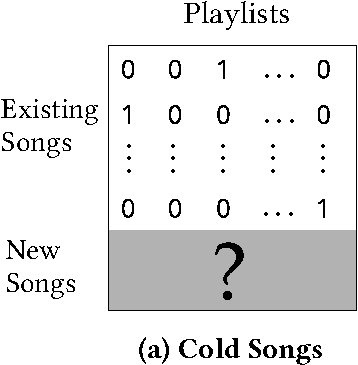
\includegraphics[width=.73\linewidth]{fig/fig_nsr.pdf}
%  \caption{}
  \label{fig:nsr}
\end{subfigure}%
\begin{subfigure}{.5\columnwidth}
  \centering
  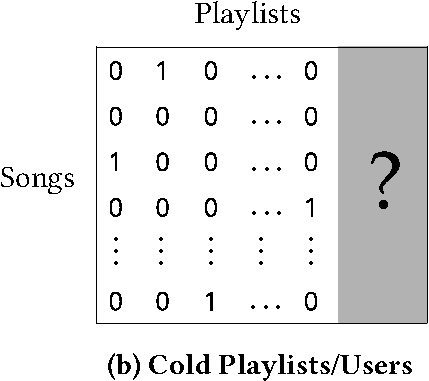
\includegraphics[width=.85\linewidth]{fig/fig_gen.pdf}
%  \caption{b}
  \label{fig:gen}
\end{subfigure}
\caption{Illustration of three cold-start settings}
\label{fig:settings}
\end{figure}



\subsection{Related work}
\section{Related work}
\label{sec:related}
% related work
% describe each task with related work: the same, the different
% describe that we don't use the order of songs, conflicting findings in literature
% mainly two pieces of work:
% - music recommendation
% - playlist generation
%{\it Some related work.}


{\bf Problem type}.
\begin{itemize}
\item playlist generation given seed (\eg a seed song, artist etc.)
\item next song recommendation, given an incomplete playlist with numerous tracks, recommend the next track that the user likely to listen.
\item another closely related task is playlist continuation, given an incomplete playlist with a few tracks, recommend a list of tracks for continuing that playlist.
\end{itemize}


{\bf Method}.
\begin{itemize}
\item Markov chain based approaches + stochastic process based (\ie autodj)
\item closely related to MC approach is finding a path in a graph (\ie kdd'12) or hypergraph (\ie aotm2011)
\item ranking based, especially popularity has been proved to be very informative, further, 
artist info has been combined with popularity in (msd paper) and (cagh paper) proposed to weighting popularity by the collocation of artists, 
achieving even better performance.
\end{itemize}


{\bf Information used}.
\begin{itemize}
\item content data such as acoustic features extracted from the audio waves of songs, lyrics, genre to be shown very informative
\item artist info
\item metadata from the interaction between users and songs, such as popularity, usage stats (groove paper), generally learn latent feature 
by collaborative filtering or family of matrix factorisation techniques.
\item order of tracks in playlist, no consensus in research community, some (a few papers) report the order info is crucial to achieve high quality recommendation,
others (another bunch of papers) found the effects of track order in playlist were negligible.
Mention that we treat playlist as a set of songs in this work, and defer the investigation of track order in playlist as future work.
\end{itemize}


{\bf Problems investigated in this paper}.
\begin{itemize}
\item given a known user (a user whom we have observed a few playlists), recommend a set of songs
\item given a new user (the recsys does not have any information about the user), recommend a set of songs
\item given a set of newly released songs, recommend songs to augment current playlists.
\end{itemize}

{\bf Methods proposed}.
Two ostensibly different but in fact closely related methods,
each one can address all three tasks.
\begin{itemize}
\item classification by focusing at positive examples
\item ranking by focusing at the top
\end{itemize}




\paragraph{Gaussian process}
The AutoDJ system~\cite{platt2002learning} automatically generate playlists given one or more seed songs, 
it learns user preference from song metadata using Gaussian Process Regression,
and generates playlist with songs similar to the seed.


\paragraph{Markov chain approaches}
Playlists are modelled as random walks in a graph where vertices are songs 
and edges represents affinities between a song pairs~\cite{mcfee2011natural}.
This model can be generalised such that edges present groups of songs (by genre, user preference etc.),
which forms a hyper-graph, and a playlist is a random walk in the hyper-graph~\cite{mcfee2012hypergraph}.

The latent Markov embedding algorithm~\cite{chen2012playlist}
learns representations of songs in a latent space in which playlists are modelled as Markov chains,
playlists are then generated by sampling a paths in the latent space from locations specified by user.

\paragraph{Popularity based ranking}
Due to the \emph{long tail} distribution of songs in playlists~\cite{aoscar2010music},
similar to many applications for recommender system, 
a popularity based approach can in fact be comparably competitive~\cite{cremonesi2010performance}.
Popularity has been combined with artist information to provide strong baselines 
for playlist generation~\cite{mcfee2012million,bonnin2013evaluating,bonnin2015automated}.

\paragraph{Review}
A nice survey and review of various approaches for playlist generation~\cite{bonnin2015automated}.


\paragraph{Next song recommendation}
Next song recommendation~\cite{jannach2015beyond} approach that first scoring each song by a number of features
(\eg acoustic features, user preference of artists, social tags, song co-occurrence in playlists etc.),
then fine-tune the ranks of top-scoring songs which hopefully make the recommended next song be a coherent continuation of user's listening history.

Groove radio~\cite{ben2017groove} uses a classification approach to sequentially recommend 
the next song by predicting the probability of each possible song for a specific user, given an artist as seed.
It makes use of various information such as song metadata, usage statistics, acoustic features, popularity of song and artist,
to build features by taking into consideration of user's listening history and the playlist seed (\ie specified artist and user).
Further, this approach can deal with a cold user or artist by falling back higher levels thanks to its hierarchical architecture.


In this paper, we describe two variants of the playlist recommendation problem,
one is augmenting a playlist by recommending a subset of songs from a collection of music $\SCal$,
given the first $K$ seed songs, where $K$ can be any positive integer from 1 to the total number of songs in playlist minus 1.
% in contrast to settings where all songs except the last one are observed\cite{}, or giving a fixed number of seed songs\cite{}.
Another variant is restricting that all songs to recommend are not observed during learning,
\ie in the setting of recommending newly released songs to augment a given playlist, which is an instance of the cold-start problem.
We call the first variant \emph{playlist augmentation} and the second \emph{new song recommendation}.

